\subsection{Android}
Utilizaremos el sistema operativo Android como entorno para implementar 
nuestra aplicación.
Android es un sistema operativo cuyo núcleo está basado en Linux,
 sistema libre, gratuito y multiplataforma.El sistema operativo fue 
desarrollado en Octubre de 2003 por Android Inc., y posteriormente
 comprado por Google en 2005.
Aunque principalmente fue diseñado para dispositivos móviles con
 pantalla táctil como teléfonos inteligentes o tablets, actualmente
también se utiliza para dispositivos wearables, televisiones e incluso
 para automóviles.  

Android permite realizar aplicaciones en un lenguaje basado en Java 
que utiliza como JVM (Java Virtual Machine) ART. Su predecesor es Dalvik~\cite{ART}.


Esta máquina virtual proporciona una serie de mejoras respecto a la jvm habitual de java:
\begin{enumerate}
\item	Compilación AOT (Ahead-of-time): Compila utilizando la herramienta dex2oat.
 Mejora el rendimiento y minimiza el tiempo de instalación de aplicaciones.
\item	Mejora el recolector de basura.
\item	Mejoras para el desarrollo y la depuración:
\begin{enumerate}
\item	Soporta perfiles de pruebas
\item	Añade nuevas características para depurar, particularmente en el monitor
 de recursos y el recolector de basura
\item	Mejoras en la descripción de los errores, añadiendo detalles 
como por ejemplo, información relativa a la actividad que intentaba
 realizar antes de un error de tipo java.lang.NullPointerException
\end{enumerate}
\end{enumerate}

ART nos proporciona un lenguaje de programación con acceso 
de una forma sencilla a las funcionalidades del teléfono 
(como GPS, llamadas, agenda, etc.).

Entre las características más importantes de este sistema operativo,
 es que tiene licencia Open Source, es decir, tanto el código fuente 
como los archivos binarios pueden ser modificados y redistribuidos
 libremente, sin tener que pagar al autor original. Esto lo hace muy
 popular entre fabricantes y desarrolladores, ya que los costes 
disminuyen mucho a la hora de lanzar un teléfono o realizar una aplicación.
	\subsubsection{Arquitectura Android}
En este apartado vamos a ver una visión global por capas de la
 arquitectura empleada por Android. Cada una de estas capas utiliza
 servicios ofrecidos por las anteriores, y ofrece a su vez los suyos 
propios a las capas de niveles superiores, tal y como podemos ver
 en la siguiente figura.
\begin{figure}[h]
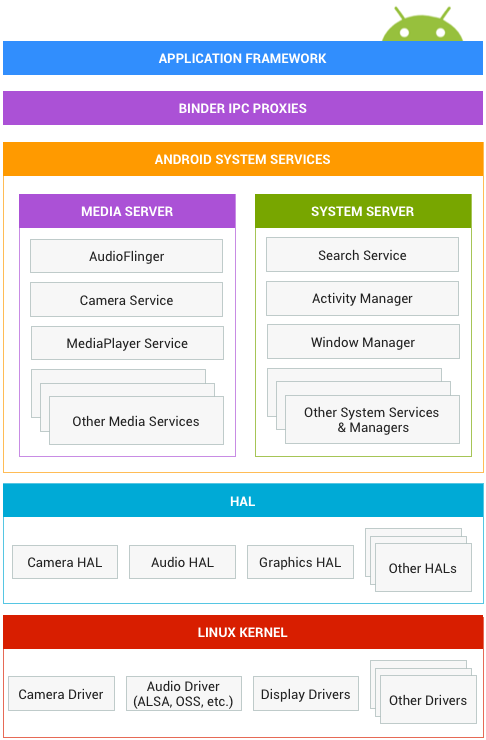
\includegraphics[scale=0.5]{arquitectura_android.png} 
\caption{Arquitectura del sistema Android.}
\end{figure}


\begin{enumerate}
\item	Aplicaciones: Este nivel contiene, tanto las incluidas por defecto 
de Android como aquellas que el usuario vaya añadiendo posteriormente,
 ya sean de terceras empresas o de su propio desarrollo. 
Todas estas aplicaciones utilizan los servicios, las API y
 librerías de los niveles anteriores. 
\item	Framework de Aplicaciones: Representa fundamentalmente el
 conjunto de herramientas de desarrollo de cualquier aplicación. 
Toda aplicación que se desarrolle para Android, ya sean las propias 
del dispositivo, las desarrolladas por Google o terceras compañías,
 o incluso las que el propio usuario cree, utilizan el mismo conjunto
 de API y el mismo "framework", representado por este nivel. 
Entre las API más importantes ubicadas aquí, se pueden encontrar las siguientes:
\begin{enumerate}
\item	Activity Manager: Conjunto de API que gestiona el ciclo de vida de
 las aplicaciones en Android.
\item	Window Manager: Gestiona las ventanas de las aplicaciones y
 utiliza la librería Surface Manager.
\item	Content Provider: Permite a cualquier aplicación compartir sus
 datos con las demás aplicaciones de Android. Por ejemplo, gracias a 
esta API la información de contactos, agenda, mensajes, etc. 
será accesible para otras aplicaciones.
\item	View System: Proporciona un gran número de elementos para poder
 construir interfaces de usuario (GUI), como listas, mosaicos, 
botones, "check-boxes", tamaño de ventanas, control de las
 interfaces mediante teclado, etc. Incluye también algunas vistas
 estándar para las funcionalidades más frecuentes.
\item	Notification Manager: Mediante el cual las aplicaciones,
 usando un mismo formato, comunican al usuario eventos que
 ocurran durante su ejecución: una llamada entrante, un mensaje recibido,
 conexión Wifi disponible, ubicación en un punto determinado, etc. 
Si llevan asociada alguna acción, en Android denominada Intent,
(por ejemplo, atender una llamada recibida) ésta se activa mediante un simple clic.
\item	Package Manager: Permite obtener información sobre los
 paquetes instalados en el dispositivo Android, además de
 gestionar la instalación de nuevos paquetes 
\item	Telephone Manager: Incluye todas las API vinculadas
 a las funcionalidades propias del teléfono (llamadas, mensajes, etc.).
\item	Resource Manager: Permite gestionar los elementos
 (cadenas de texto traducidas a diferentes idiomas, imágenes, sonidos o layouts)
 que forman parte de la aplicación y que están fuera del código.
\item	Location Manager: Posibilita a las aplicaciones la obtención
 de información de localización y posicionamiento.
\end{enumerate}
\item XMPP Service: Colección de API para utilizar este protocolo
 de intercambio de mensajes basado en XML. 
\item	Librerías: La siguiente capa se corresponde con las librerías
 utilizadas por Android. Estas han sido escritas utilizando C/C++ y
 proporcionan a Android la mayor parte de sus capacidades 
más características. Junto al núcleo basado en Linux, estas librerías 
constituyen el corazón de Android.
Entre las librerías más importantes ubicadas aquí, se pueden
 encontrar las siguientes:
\begin{enumerate}
\item	Surface Manager: Es la encargada de componer los 
diferentes elementos de navegación de pantalla. Gestiona
 también las ventanas pertenecientes a las distintas
 aplicaciones activas en cada momento.
\item	Media Framework: Proporciona todos los códecs necesarios 
para el contenido multimedia soportado en Android (vídeo, audio,
 imágenes estáticas y animadas, etc.)
\item	SQLite: Creación y gestión de bases de datos relacionales.
\item	OpenGL/SL y SGL: Representan las librerías gráficas y,
 por tanto, sustentan la capacidad gráfica de Android.
 OpenGL/SL maneja gráficos en 3D y permite utilizar,
 en caso de que esté disponible en el propio dispositivo móvil,
 el hardware encargado de proporcionar gráficos 3D.
 Por otro lado, SGL proporciona gráficos en 2D,
 por lo que será la librería más habitualmente utilizada por
 la mayoría de las aplicaciones. Una característica importante
 de la capacidad gráfica de Android es que es posible 
desarrollar aplicaciones que combinen gráficos en 3D y 2D.
\item	FreeType: Permite trabajar de forma rápida y
 sencilla con distintos tipos de fuentes.
\item	WebKit: Proporciona un motor para las aplicaciones
 de tipo navegador y forma el núcleo del actual navegador
 incluido por defecto en la plataforma Android.
\item	SSL: Posibilita la utilización de dicho protocolo para
 establecer comunicaciones seguras.
\item	Libc: Incluye todas las cabeceras y funciones según
 el estándar del lenguaje C. Todas las demás librerías se 
definen en este lenguaje.
\end{enumerate}
\item	Tiempo de ejecución de Android: Al mismo nivel que las
 librerías de Android se sitúa el entorno de ejecución.
 Éste lo constituyen las Core Libraries, que son librerías con
 multitud de clases Java y la máquina virtual ART~\cite{ART}.
\item Núcleo Linux: Android utiliza el núcleo de Linux como una 
capa de abstracción para el hardware disponible en los dispositivos
 móviles. Esta capa contiene los drivers necesarios para que cualquie
r componente hardware pueda ser utilizado mediante las llamadas
 correspondientes. Siempre que un fabricante incluye un nuevo
 elemento de hardware, lo primero que se debe realizar para que 
pueda ser utilizado desde Android es crear las librerías de control
 o drivers necesarios dentro de este kernel de Linux embebido 
en el propio Android. 
\end{enumerate}
\subsubsection{Componentes Android}
Existen cinco componentes importantes en las aplicaciones Android

\begin{figure}[h]
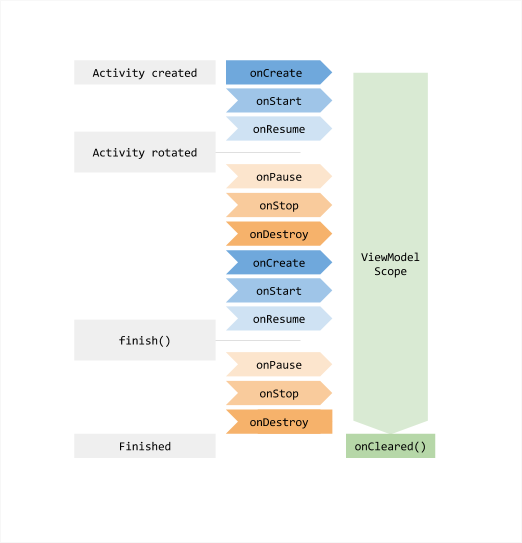
\includegraphics[scale=0.50]{ciclo_de_vida.png} 
\caption{Ciclo de vida de una aplicación Android.}
\end{figure}
\begin{enumerate}

\item	Activity: Se puede decir que una actividad es cada una de
 las pantallas que nosotros mostramos en la ejecución de nuestra 
aplicación. Cada actividad puede encontrarse en diferentes estados:
\begin{enumerate}
\item	onCreate: Representa el momento en que se crea la actividad
\item	onStart: Es donde la actividad se muestra en pantalla.
\item	onRestart: Cuando una aplicación estaba parada y la volvemos a activar.
\item	onResume: La actividad va a empezar a responder a la interacción del usuario.
\item	onPause: La actividad va a dejar de responder a la interacción del usuario.
\item	onStop: Cuando la actividad pasa a segundo plano.
\item	onDestroy: Cuando se destruye una actividad y se liberan sus recursos.
\end{enumerate}




Una actividad consta de dos partes:
\begin{enumerate}
\item	La parte lógica: se trata de un archivo java donde se manipula,
 interactúa y coloca el código de la actividad
\item	La parte gráfica: Se trata de un XML donde se introducen los
 elementos que formarán la estructura de la pantalla.
\end{enumerate}
\item	Services: Son tareas que se ejecutan en segundo plano y no
 tienen una interfaz que vea el usuario. Se suelen utilizar para realizar 
operaciones de larga ejecución o para realizar trabajo con procesos remotos.
Se encargan de realizar tareas que deben continuar ejecutándose 
cuando nuestra aplicación no está en primer plano.
\item	Content Provider: Se trata de un mecanismo proporcionado
 por la plataforma Android para permitir compartir información entre 
aplicaciones. Se permite acceder al sistema de ficheros, bases de 
datos SQLite, la información se encuentran la lista de contactos, la 
aplicación de SMS, o el calendario/agenda.  
\item	Intent: Son objetos que se utilizan para arrancar actividades o 
servicios, o enviar eventos a múltiples destinatarios. Estos objetos 
también se pueden utilizar para realizar paso de mensajes entre 
actividades de la misma aplicación o entre distintas aplicaciones.
Broadcast Receiver: Un broadcast es un mensaje que cualquiera 
aplicación puede recibir. Estos mensajes broadcast pueden ser 
un reinicio del dispositivo, aviso de batería baja o al conectar el
 móvil a un cargador. Con este componente se puede configurar
 el recibir ese broadcast y que nuestra aplicación haga alguna acción 
determinada en ese momento.
\end{enumerate}
\subsubsection{Estructura de una aplicación Android}
En este apartado vamos a explicar la estructura de los componentes
 que tiene una aplicación Android.
\begin{enumerate}
\item	Src: En esta carpeta se introducen los archivos java 
que componen nuestra aplicación.
\item	Gen: Dentro de esta carpeta hay un archivo llamado “R.java” 
donde se guardan los identificadores de todos los componentes
 utilizados en la aplicación.
\item	Libs: Se encuentran librerías externas que necesita el proyecto.
\item	Res: En este directorio se encuentran todos los recursos
 de la aplicación.
\item	Res/drawable: En esta carpeta se guardan las imágenes 
que vamos a utilizar en nuestra aplicación.
\item	Res/layout: Carpeta donde se guardan los XML de las actividades.
\item	Res/values: Carpeta donde se guarda el archivo “strings.xml”,
 el cual almacena las cadenas de texto que utilizaremos en la aplicación. 
AndroidManifest.xml: Este archivo es el más importante de la aplicación
 y lo vamos a describir con más detalle en el siguiente apartado.
	Android Manifest
Éste archivo se considera el más importante de la aplicación ya que es
 donde se declaran todas las actividades de la aplicación, los permisos,
 versiones del SDK que usamos, etc.
 
En la primera línea se indica la versión y el formato del documento:
 
La etiqueta principal es <manifest> y tiene varios atributos:
\begin{enumerate}
\item[Xmlns]: lo coloca Eclipse por defecto.
\item[Package]: Hace referencia al nombre del paquete de la aplicación.
\item[VersionCode]: Es el número de versión del código de la aplicación
\item[VersionName]: También es el número de la versión
 \end{enumerate}
 
La etiqueta SDK se configura para saber la compatibilidad de las 
versiones en Android.
\begin{enumerate}
\item minSDKVersion: Indica la versión mínima de SDK para que funcione
 nuestra aplicación.
\item targetSdkVersion: Es la versión de la API a la que se dirige
 principalmente la aplicación.
\end{enumerate}
La etiqueta <uses-permission> se utiliza para dar permisos a la aplicación.
En nuestro caso, hemos configurado para que nuestra aplicación
pueda acceder a internet, pueda acceder al GPS y pueda escribir 
en un almacenamiento externo.
 
Dentro de la etiqueta <application> se introducen todos los 
elementos que componen la aplicación.
\begin{enumerate}
\item allowBackup: Con el valor "true" se le permite al sistema 
hacer copia de seguridad de la aplicación y del contenido.
\item Icon: Es el icono de la aplicación.
\item Label: Es el nombre de la aplicación.
\item Theme: Es el estilo de la aplicación.
\end{enumerate}
En la etiqueta <activity> es donde se dan de alta todas las 
actividades que vamos a tener en la aplicación.
\begin{enumerate}
\item Name: Contiene el nombre de la clase java que implementa el activity.
\item Label: Es el nombre de la activity.
\end{enumerate}
<Intent-filter> indica lo que la activity tiene permitido hacer.
\end{enumerate}